
\section{Motivation}

\subsection{Cyclus Foundations}\label{intro:cyc}

Deciding how a simulation is structured from an interactions standpoint is a
delicate balance of known necessity and perceived future needs. There are basic
decisions to make, such as modeling material transfer as discrete or
continuous. Discrete transfers more closely match reality and may provide
insights in that regard, however they require more of their modeling apparatus
due to messaging needs and other structures. More complex decisions include how
one wants to determine connections between facilities, and whether such
connections are assigned statically and incorporated into the simulation
architecture or determined dynamically. Guerin's comment
in \S\ref{sec:litrev-benchmarks} stems from this ``freedom''. These
simulation-engine decisions comprise the art-related portion of fuel cycle
simulation, but developers have a goal of making these decisions in as informed
a way as possible using domain-level knowledge with respect to our known and
perceived requirements. In general, this work tries to minimize the sheer number
of choices we make in this regard, instead relying on well known and well
documented practices of computer scientists and systems engineers.

The \Cyclus team is also interested in fostering a user and developer ecosystem.
Accordingly, such concerns also drive the simulation architecture design. The
agent-based nature of \Cyclus provides an opportunity to reduce barriers to
entry into the ecosystem. Given a few basic tenets of agent interaction, other
developers should be able to create a new agent to ``plug in'' to the
simulation. Intuitively, a minimal set of behaviors must be defined to
sufficiently inform the simulation infrastructure to run the simulation. This
freedom allows the simulation program introduce agents at run time, effectively
separating the simulation engine's functionality from the agents in the
simulation.

Such a framework provides many benefits. First, there is a clear separation of
concerns. The \Cyclus core is concerned with modeling system dynamics whereas
individual agents are concerned with domain-specific issues. Accordingly,
developers can focus their attention appropriately, focusing either on the core
code base or on agent development. Separating agent development from core
development also allows \Cyclus to remain a viable open-source candidate to
model nuclear fuel cycle dynamics. Because domain-level information is
incorporated into agent libraries which are dynamically loaded at runtime, a
closed-source developer can focus their efforts entirely on developing agent
libraries. Furthermore, developers could participate both privately and
publicly, e.g., adding general capability to the \Cyclus core that is needed for
some functionality without specifying the internals. Such a community paradigm
is shown in Figure \ref{fig:community}.

\begin{figure}[htbp!]
  \begin{center}
    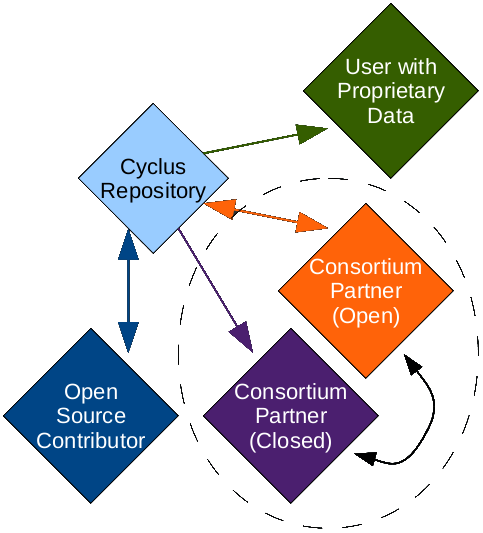
\includegraphics[height=8cm]{./figs/community.png}
  \end{center}
  \caption{The Cyclus Participation Paradigm} 
  \label{fig:community}
\end{figure}

In order to develop and maintain the core code separate from the agent modules,
well-defined interactions must be provided between agents and the \Cyclus
core. The remaining part of the section provides a proposal for such
interactions that allow for a variety facility deployment and supply-demand
matching algorithms to be employed. A description of the market resolution
interface is provided, and basic agent simulation interaction, such as entering
and leaving the simulation is also described.

In the absence of supply constraints, aggregated
individual facility behavior and fleet-based models are equivalent. However, any
system in which recycling exists will, by definition, have some supply
constraints.

\subsection{Statement of Work}
